\subsubsection{Physical Layer - Inverse Kinematics Verifier}
As detailed in design section \ref{IKDESIGN}, the implemented Inverse Kinematics Verifier uses an analytical solution to calculate the manipulator joint angles required to position the end-effector at a specified location. Initially, an analytical formula was developed specifically for the Automata EVA arm (details in \nameref{evaSpecSheet}) available in the lab. This limited the compatibility of the reconfiguration planner to only that specific manipulator.
\\\\
To increase compatibility, a Unified Robotics Description Format (URDF) file was created for the Automata EVA, as shown in \nameref{evaURDF}. The IKPy package \cite{ikpy} was then used to generate an analytical solution for use by the Inverse Kinematics Verifier and Motion Planner. Users can now update the reconfiguration planner to work with different mobile manipulators by simply replacing or modifying the URDF file.
\\\\
The inverse kinematics verifier is used to ensure that the start and final position of each module movement in the reconfiguration semantic solution is reachable by the mobile manipulator. In the case of a module being out of reach, the verifier returns the state transition that caused the failure. Otherwise, the semantic solution is sent to the motion planner for further processing.

\subsubsection{Physical Layer - Robot Description File}
\begin{figure}[H]
	\centering
	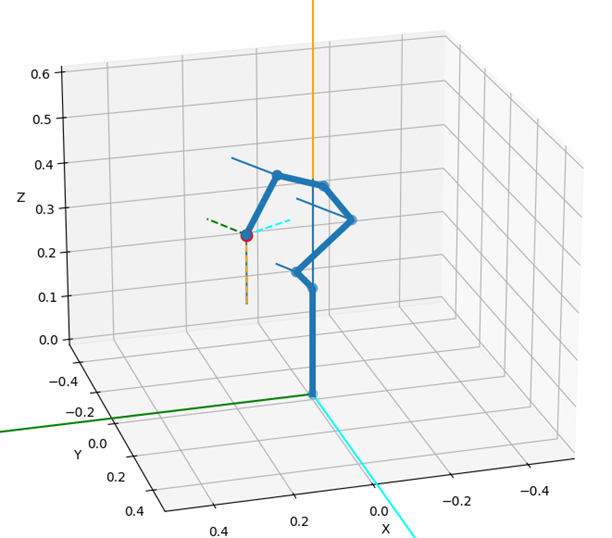
\includegraphics[width=\textwidth]{IK.png}
	\caption{Automata EVA Kinematics Visualisation}
	\label{EvaIKbasic}
\end{figure}
A URDF file is used to define the mechanical structure, dimensions, joint configurations, and physical constraints of the mobile manipulator the physical layer is simulating to verify the logic layers semantic solution. URDF files are an XML-based file format that is widely used in robotics \cite{urdfProof} to describe robots to software systems. The file describes a robot as a collection of links and joints that can articulate around each other according to specified constraints. URDF files are also modular meaning they can include other URDF files, aiding in the design of particularly complex robots. This for example means that a user can develop a URDF file for an arm end-effector and simply include it in the already existing arm file to attach it to the arm. 
URDF files also allow for the visualization of the defined arm joints, as seen in figure \ref{EvaIKbasic} which can be overlaid on top of our module state display to visualise mobile manipulator pose on the modular space system. Additionally available online packages such as urdf-loader \cite{urdfLoader} can display the visual meshes described in the URDF file to view the mobile manipulator in more detail such as seen in figure \ref{EvaIKadvanced}.
\begin{figure}[H]
	\centering
	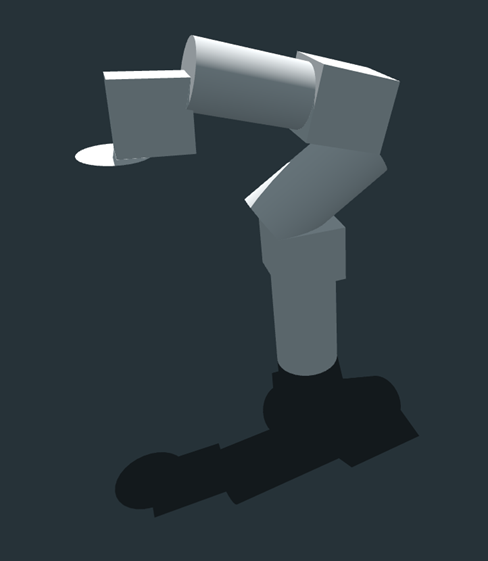
\includegraphics[width=0.8\textwidth]{IKmodel.png}
	\caption{Automata EVA URDF Model Visualisation created through urdf-loader \cite{urdfLoader}}
	\label{EvaIKadvanced}
\end{figure}

\subsubsection{Physical Layer - Motion Planner}
Due to time constraints during the project, instead of implementing an advanced motion planner, a simple motion planner was implemented that makes assumptions based on the lab environment surrounding the mobile manipulator available in the lab. Physical constraints of the robot arm and the environment are applied to the system during module movements using 2 basic rules:
\begin{enumerate}[]
	\item Modules can only be picked up by the mobile arm if no blocks are above them.
	\item Modules can only be placed at a supported position (above another module and on the ground) and cannot be placed at negative z values (below the ground)
\end{enumerate}
The combination of these two rules applies the physical constraints of gravity and the presence of the ground. If either rule is broken, the planner returns the state transition causing the failure. Otherwise, it generates and returns an instruction set in the form of an array containing each manipulator action sequentially required to perform the state reconfiguration. The available instructions the motion planner can generate can be seen in Figure \ref{instructions}

\begin{figure}[H]
	\begin{tabularx}{\textwidth} {| p{0.16\textwidth} | p{0.14\textwidth} | X |}
		\hline
		\textbf{Instruction} & \textbf{Information} & \textbf{Action}\\
		\hline
		CONNECT 	 & None	& Signal the arms end-effector to grab/connect\\
		\hline
		DISCONNECT   & None & Signal to the arms end-effector to drop/disconnect\\
		\hline
		MOVE TO 	 & Position, Joint angles & Move the arm to position the end-effector at the supplied position by transitioning the arms joint angles to the supplied joint angles\\
		\hline
	\end{tabularx}
	\caption{Instructions available to the Physical Layer Motion Planner}
	\label{instructions}
\end{figure}

